\chapter{Particle Physics}
\begin{abox}
	Practise set-2
\end{abox}
\begin{enumerate}
	\item Q1. Which one of the following sets corresponds to fundamental particles?
	 {\exyear{ 	GATE-2012}}
	 \begin{tasks}(2)
		\task[\textbf{a.}]Proton, electron and neutron
		\task[\textbf{b.}]Proton, electron and photon
		\task[\textbf{c.}]Electron, photon and neutrino
		\task[\textbf{d.}]Quark, electron and meson 
	\end{tasks}
\begin{answer}
So the correct answer is \textbf{Option (a)}
\end{answer}
	\item Q2. Choose the CORRECT statement from the following
	 \begin{tasks}(1)
		\task[\textbf{a.}]Neutron interacts through electromagnetic interaction
		\task[\textbf{b.}]Electron does not interact through weak interaction
		\task[\textbf{c.}]Neutrino interacts through weak and electromagnetic interaction
		\task[\textbf{d.}] Quark interacts through strong interaction but not through weak interaction
	\end{tasks}
\begin{answer}
	So the correct answer is \textbf{Option (d)}
\end{answer}
	\item Q3. The isospin and the strangeness of $\Omega^{-}$baryon are
	{\exyear{ GATE-2011}}
	 \begin{tasks}(4)
		\task[\textbf{a.}]$1,-3$
		\task[\textbf{b.}]$0,-3$
		\task[\textbf{c.}]1,3
		\task[\textbf{d.}]0,3 
	\end{tasks}
\begin{answer}
	So the correct answer is \textbf{Option (b)}
\end{answer}
	\item Q4. The isospin $(I)$ and baryon number $(B)$ of the up quark is
	{\exyear{ 	GATE-2013}}
	 \begin{tasks}(2)
		\task[\textbf{a.}]$I=1, B=1$
		\task[\textbf{b.}]$I=1, B=1 / 3$
		\task[\textbf{c.}]$I=1 / 2, B=1$
		\task[\textbf{d.}]$I=1 / 2, B=1 / 3$ 
	\end{tasks}
\begin{answer}
	So the correct answer is \textbf{Option (d)}
\end{answer}
	\item Q5. Which one of the following is a fermions'?
	{\exyear{ 	GATE-2014}}
	 \begin{tasks}(2)
		\task[\textbf{a.}]$\alpha$-particle
		\task[\textbf{b.}]${ }_4 B e^7$ nucleus
		\task[\textbf{c.}]Hydrogen atom
		\task[\textbf{d.}]Deuteron 
	\end{tasks}
\begin{answer}
	If a nucleus contains odd number of nucleons, it is fermions. If a nucleus contains even number of nucleons, it is a boson.\\
	So the correct answer is \textbf{Option (b)}
\end{answer}
	\item Q6. In the decay, $\mu^{+} \rightarrow e^{+}+v_e+X$, what is $X$ ?
	{\exyear{ GATE-2018}}
	 \begin{tasks}(4)
		\task[\textbf{a.}]$\gamma$
		\task[\textbf{b.}]$\bar{v}_e$
		\task[\textbf{c.}]$v_\mu$
		\task[\textbf{d.}]$\bar{v}_\mu$ 
	\end{tasks}
\begin{answer}
	\begin{align*}
	u^{+} \rightarrow e^{+}+v_e+\bar{v}_u\\
	\begin{array}{rrrrr}
	L_u: & -1 & 0 & 0 & -1 \\
	L_e: & 0 & -1 & +1 & 0
	\end{array}
	\end{align*}
	So the correct answer is \textbf{Option (d)}
\end{answer}
	\item Q7. The basic process underlying the neutron $\beta$-decay is
	{\exyear{ GATE-2010}}
	 \begin{tasks}(2)
		\task[\textbf{a.}]$d \rightarrow u+e^{-}+\bar{v}_e$
		\task[\textbf{b.}]$d \rightarrow u+e^{-}$
		\task[\textbf{c.}]$s \rightarrow u+e^{-}+\bar{v}_e$
		\task[\textbf{d.}]$u \rightarrow d+e^{-}+\bar{v}_e$ 
	\end{tasks}
\begin{answer}
	\begin{align*}
	
	\end{align*}
\end{answer}
	\item Q8. Match the reactions on the left with the associated interactions on the right.\\
	(1) $\pi^{+} \rightarrow \mu^{+}+v_\mu$\hspace{3cm}
	(i) Strong\\
	(2) $\pi^0 \rightarrow \gamma+\gamma$\hspace{3.5cm}
	(ii) Electromagnetic\\
	(3) $\pi^0+\mathrm{n} \rightarrow \pi^{-}+\mathrm{p}$\hspace{2.6cm}
	(iii) Weak
	{\exyear{ GATE-2010}}
	 \begin{tasks}(2)
		\task[\textbf{a.}]$(1$, iii), (2, ii), (3, i)
		\task[\textbf{b.}]$(1$, i), (2, ii), (3, iii)
		\task[\textbf{c.}](1, ii), (2, i), (3, iii)
		\task[\textbf{d.}](1, iii), (2, i), (3, ii) 
	\end{tasks}
	\item Q9. The quark content of $\Sigma^{+}, K^{-}, \pi^{-}$and $p$ is indicated:
	$$
	\left|\Sigma^{+}\right\rangle=|u u s\rangle ;\left|K^{-}\right\rangle=|s \bar{u}\rangle ;\left|\pi^{-}\right\rangle=|\bar{u} d\rangle ;|p\rangle=|u u d\rangle .
	$$
	In the process, $\pi^{-}+p \rightarrow K^{-}+\Sigma^{+}$, considering strong interactions only, which of the following statements is true?
	{\exyear{ GATE-2012}}
	 \begin{tasks}(1)
		\task[\textbf{a.}]The process, is allowed because $\Delta \mathrm{S}=0$
		\task[\textbf{b.}] The process is allowed because $\Delta \mathrm{I}_3=0$
		\task[\textbf{c.}] The process is not allowed because $\Delta \mathrm{S} \neq 0$ and $\Delta \mathrm{I}_3 \neq 0$
		\task[\textbf{d.}]The process is not allowed because the baryon number is violated 
	\end{tasks}
	\item Q10. The decay process $n \rightarrow p^{+}+e^{-}+\bar{v}_e$ violates
	{\exyear{ 	GATE-2013}}
	 \begin{tasks}(2)
		\task[\textbf{a.}]Baryon number
		\task[\textbf{b.}] lepton number
		\task[\textbf{c.}] Isospin
		\task[\textbf{d.}] Strangeness
	\end{tasks}
	\item Q11. Which one of the following three-quark states $(q q q)$ denoted by $X$ CANNOT be a possible baryon? The corresponding electric charge is indicated in the superscript.
	{\exyear{ 	GATE-2014}}
	 \begin{tasks}(4)
		\task[\textbf{a.}]$X^{++}$
		\task[\textbf{b.}]$\mathrm{X}^{+}$
		\task[\textbf{c.}]$X^{-}$
		\task[\textbf{d.}] $\mathrm{X}^{--}$ 
	\end{tasks}
	\item Q12. The decay $\mu^{+} \rightarrow e^{+}+\gamma$ is forbidden, because it violates
	{\exyear{ 	GATE-2015}}
	 \begin{tasks}(1)
		\task[\textbf{a.}] Momentum and lepton number conservations
		\task[\textbf{b.}]Baryon and lepton number conservations
		\task[\textbf{c.}]Angular momentum conservation
		\task[\textbf{d.}]  Lepton number conservation
	\end{tasks}
	\item Q13. In the $S U(3)$ quark model, the triplet of mesons $\left(\pi^{+}, \pi^0, \pi^{-}\right)$has
	{\exyear{ GATE-2016}}
	 \begin{tasks}(2)
		\task[\textbf{a.}]Isospin $=0$, Strangeness $=0$
		\task[\textbf{b.}] Isospin $=1$, Strangeness $=0$
		\task[\textbf{c.}]Isospin $=\frac{1}{2}$, Strangeness $=+1$
		\task[\textbf{d.}]  Isospin $=\frac{1}{2}$, Strangeness $=-1$
	\end{tasks}
	\item Q14. Which one of the following conservation laws is violated in the decay $\tau^{+} \rightarrow \mu^{+} \mu^{+} \mu^{-}$
	{\exyear{ GATE-2017}}
	 \begin{tasks}(2)
		\task[\textbf{a.}]Angular momentum
		\task[\textbf{b.}]Total Lepton number
		\task[\textbf{c.}]Electric charge
		\task[\textbf{d.}]Tau number 
	\end{tasks}
	\item Q15. The elementary particle $\Xi^0$ is placed in the baryon decuplet, shown below, at
		{\exyear{GATE-2018}}
	\begin{figure}[H]
		\centering
		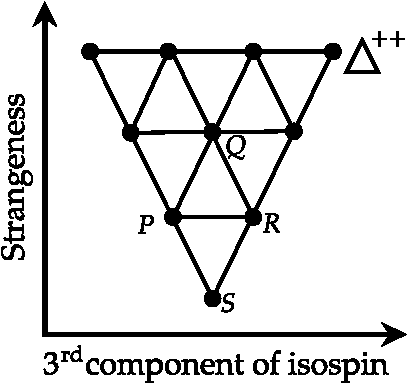
\includegraphics[height=4cm,width=4.5cm]{NP-13}
	\end{figure}
	 \begin{tasks}(4)
		\task[\textbf{a.}]$P$
		\task[\textbf{b.}]$Q$
		\task[\textbf{c.}]$R$
		\task[\textbf{d.}] $S$ 
	\end{tasks}
	\item Q16. Considering baryon number and lepton number conservation laws, which of the following process is/are allowed?
	(i) $p \rightarrow \pi^0+e^{+}+v_e$\hspace{2cm}
	(ii) $e^{+}+v_e \rightarrow \mu^{+}+v_\mu$
	{\exyear{ 	GATE-2019}}
	 \begin{tasks}(2)
		\task[\textbf{a.}]Both (i) and (ii)
		\task[\textbf{b.}]Only (i)
		\task[\textbf{c.}]Only (ii)
		\task[\textbf{d.}]Neither (i) nor (ii)
	\end{tasks}
	\item Q17. A massive particle $X$ in free space decays spontaneously into two photons. Which of the following statements is true for $X$ ?
{\exyear{ 	GATE-2019}}
	 \begin{tasks}(2)
		\task[\textbf{a.}] $X$ is charged
		\task[\textbf{b.}]Spin of $X$ must be greater than or equal to 2
		\task[\textbf{c.}]$X$ is a boson
		\task[\textbf{d.}]$X$ must be a baryon 
	\end{tasks}
	\item Q18. Low energy collision ( $s$-wave scattering) of pion $\left(\pi^{+}\right)$with deuteron $(d)$ results in the production of two proton $\left(\pi^{+}+d \rightarrow p+p\right)$. The relative orbital angular momentum (in units of $\hbar$ ) of the resulting two-proton system for this reaction is
	{\exyear{ GATE-2019}}
	 \begin{tasks}(4)
		\task[\textbf{a.}]0
		\task[\textbf{b.}]1
		\task[\textbf{c.}]2
		\task[\textbf{d.}] 3
	\end{tasks}
	\item Q19. A particle $Y$ undergoes strong decay $Y \rightarrow \pi^{-}+\pi^{-}$. The isospin of $Y$ is---------
	{\exyear{ GATE- 2020}}
	\item Q20. A particle $X$ is produced in the process $\pi^{+}+p \rightarrow K^{+}+X$ via the strong interaction. If the quark content of the $K^{+}$is $u \bar{s}$, the quark content of $X$ is
{\exyear{	GATE- 2020}}
	 \begin{tasks}(4)
		\task[\textbf{a.}]$c \bar{s}$
		\task[\textbf{b.}]und
		\task[\textbf{c.}]uus
		\task[\textbf{d.}]$u \bar{d}$ 
	\end{tasks}
	
	
	
	
	
	
	
	
	
\end{enumerate}